
\section{Gantt Chart}

A Gantt chart was used to give a high-level overview of my project to give myself a realistic timetable of when different aspects had to be completed by. Figure~\ref{fig:gantt-chart-1} shows the initial Gantt chart up to the progress report and Figures~\ref{fig:gantt-chart-2} and~\ref{fig:gantt-chart-3} show the final phases of this project up to the final submission.

\begin{figure}[H]
  \centering
  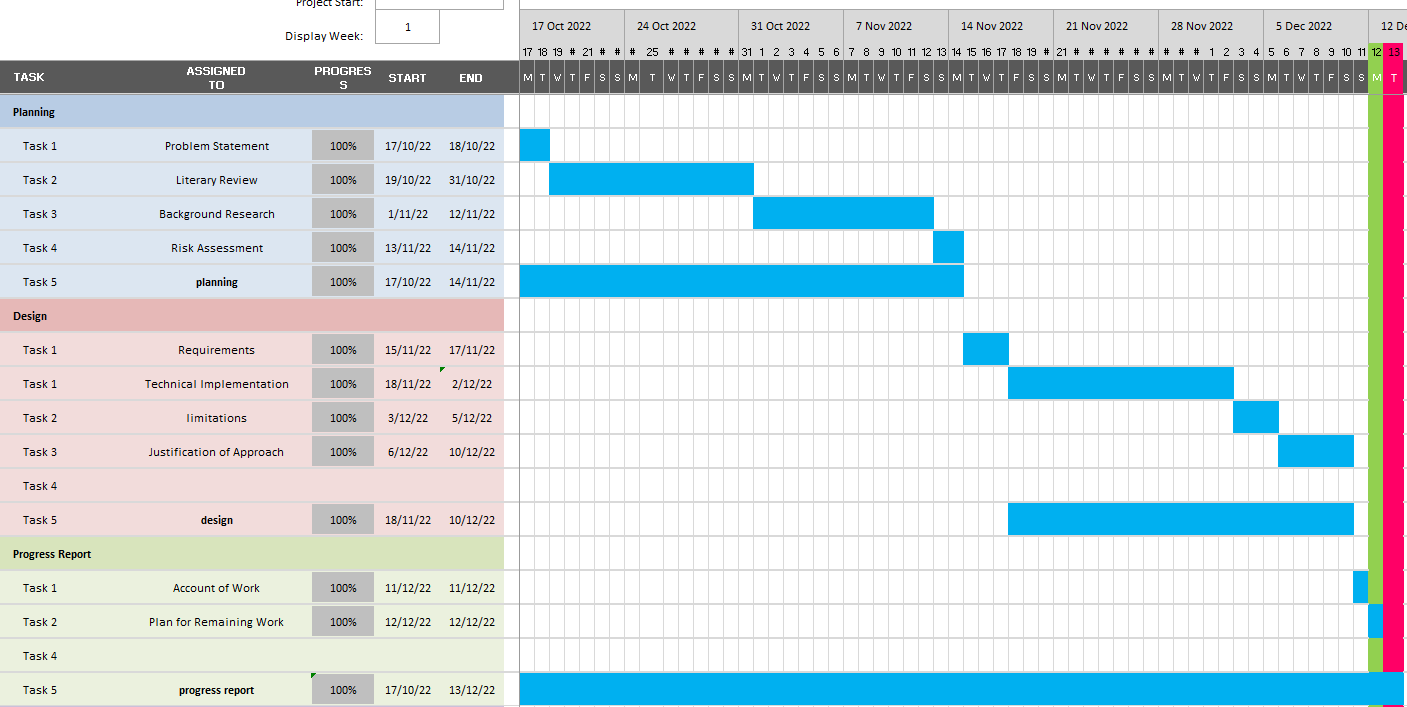
\includegraphics[width=\textwidth]{assets/images/charts/gantt/progress.png}
  \caption{Gantt Chart leading up to the progress report}
  \label{fig:gantt-chart-1}
\end{figure}

\begin{figure}[H]
  \centering
  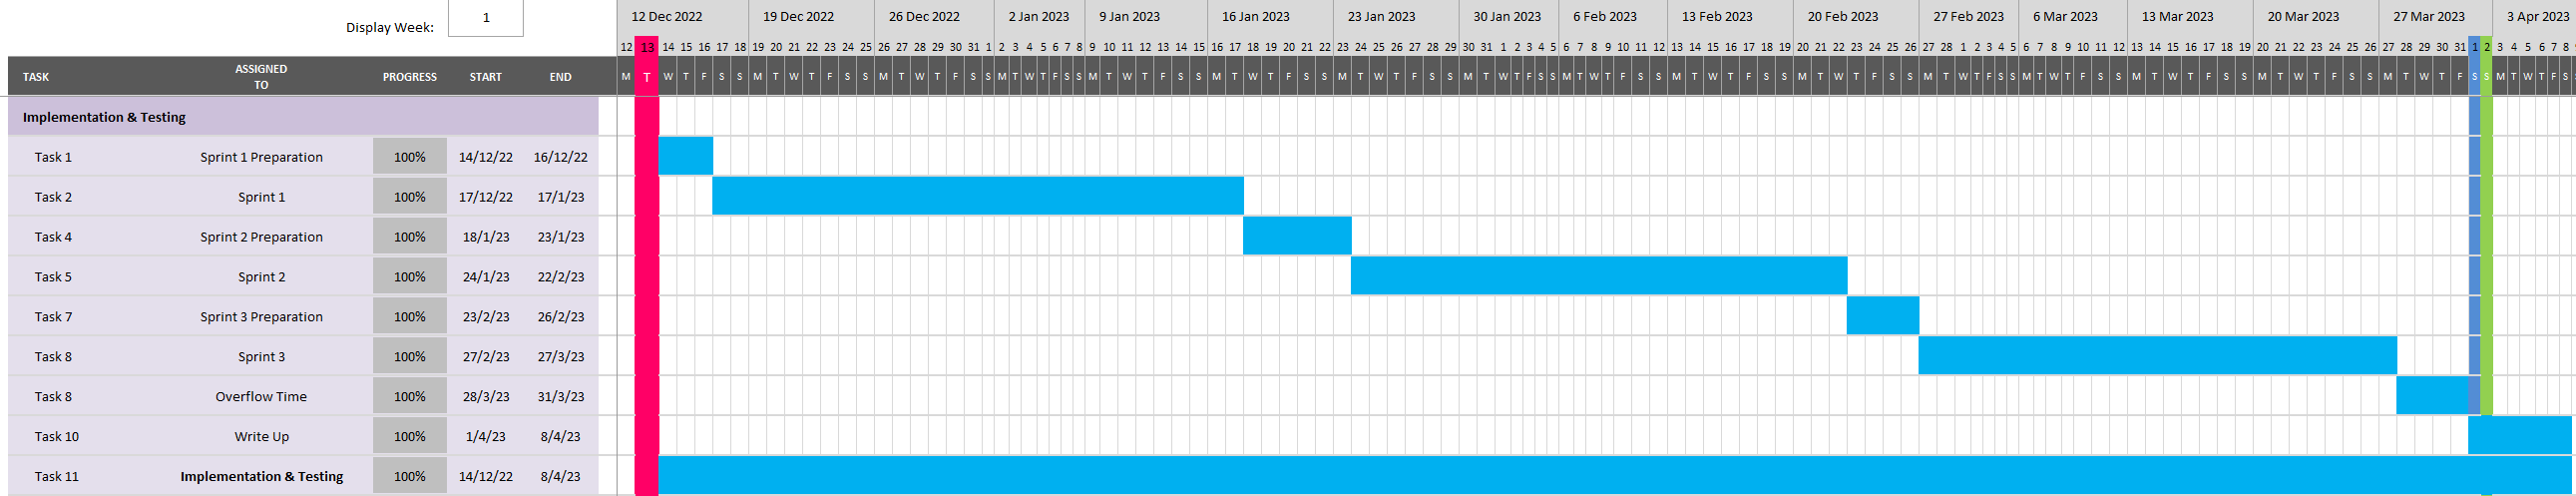
\includegraphics[width=\textwidth]{assets/images/charts/gantt/impl.png}
  \caption{Gantt Chart showing the three sprints}
  \label{fig:gantt-chart-2}
\end{figure}

\begin{figure}[H]
  \centering
  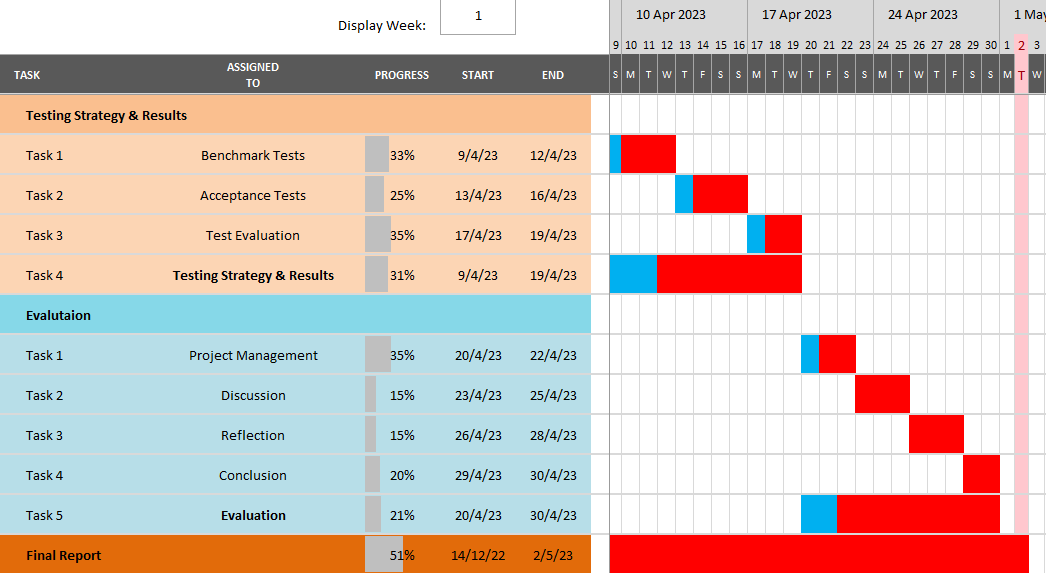
\includegraphics[width=\textwidth]{assets/images/charts/gantt/testing-eval.png}
  \caption{Gantt Chart showing the final testing and evaluation}
  \label{fig:gantt-chart-3}
\end{figure}